\documentclass{article}
\usepackage{tikz}
\usetikzlibrary{shapes.geometric, patterns}

\begin{document}

\begin{figure}[h]
    \centering
    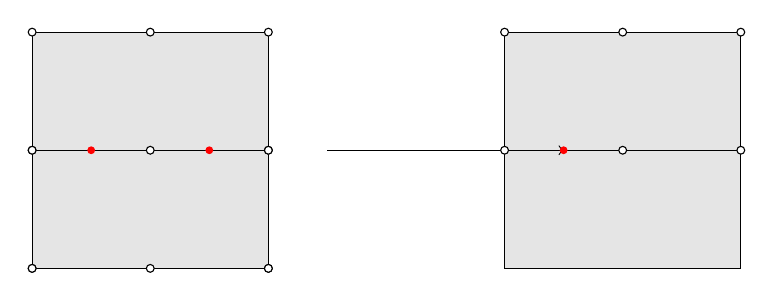
\begin{tikzpicture}[scale=1.5]

        % Drawing the first cube
        \draw[fill=black!10] (-1,-1) -- (1,-1) -- (1,1) -- (-1,1) -- cycle;
        \draw[fill=black!10] (-1,0) -- (1,0) -- (1,1) -- (-1,1) -- cycle;
        \draw[fill=black!10] (-1,0) -- (1,0) -- (1,-1) -- (-1,-1) -- cycle;
        \draw[fill=black!10] (-1,-1) -- (1,-1) -- (1,0) -- (-1,0) -- cycle;

        % Drawing the second cube
        \draw[fill=black!10] (3,-1) -- (5,-1) -- (5,1) -- (3,1) -- cycle;
        \draw[fill=black!10] (3,0) -- (5,0) -- (5,1) -- (3,1) -- cycle;
        \draw[fill=black!10] (3,0) -- (5,0) -- (5,-1) -- (3,-1) -- cycle;
        \draw[fill=black!10] (3,-1) -- (5,-1) -- (5,0) -- (3,0) -- cycle;

        % Drawing the connecting edges between the cubes
        \draw[->] (1.5,0) -- (3.5,0);

        % Drawing the red vertices inside the first cube
        \node at (-0.5,0) [circle, fill=red, inner sep=1pt]{};
        \node at (0.5,0) [circle, fill=red, inner sep=1pt]{};

        % Drawing the red vertices inside the second cube
        \node at (3.5,0) [circle, fill=red, inner sep=1pt]{};

        % Drawing the black vertices outside the cubes
        \foreach \x in {-1,...,1} {
            \foreach \y in {-1,...,1} {
                \node at (\x,\y) [circle, draw=black, fill=white, inner sep=1pt]{};
            }
        }

        % Drawing the black vertices on the top faces of both cubes
        \foreach \x in {3,...,5} {
            \foreach \y in {0,1} {
                \node at (\x,\y) [circle, draw=black, fill=white, inner sep=1pt]{};
            }
        }

        % Drawing the black vertices on the bottom faces of both cubes
        \foreach \x in {-1,1} {
            \foreach \y in {-1,0} {
                \node at (\x,\y) [circle, draw=black, fill=white, inner sep=1pt]{};
            }
        }

    \end{tikzpicture}
    \caption{A feasible set of size two (discs in red) in $\square_{i=1}^4 K_2$ and all possible extensions to a feasible set of size three (squares in black).}
    \label{fig:feasible_set_extension}
\end{figure}

\end{document}